\chapter{The experimental apparatus}
\label{chap:CMS}

\section{The \LHC}
\label{sec:LHC}

The Large Hadron Collider (\LHC)~\cite{Bruning:2004ej} at \CERN is the most powerful particle accelerator in the world, located in the same tunnel as the Large Electron-Positron collider (\LEP)~\cite{Brianti:2004qq}. At 27 km in circumference, the LHC is a two-ring, superconducting accelerator and proton-proton (or proton-ion or ion-ion) collider with a two-fold experimental mandate: to probe the electroweak symmetry breaking mechanism via which particles in the Standard Model (SM) attain mass, and to extend the exploration of the energy frontier in search for new physics beyond the SM (\BSM). Pictured in~\FigureRef{fig:LHC} is the approximate LHC ring size superimposed on top of a map of the Swiss-French border near Geneva, Switzerland. The LHC is comprised of octants, and the locations at which beam collisions occur are the interaction points (IP). The general purpose high luminosity ($L$) experiments on the LHC ring are the CMS (Compact Muon Solenoid)~\cite{Chatrchyan:2008aa} and ATLAS (A Toroidal LHC ApparatuS)~\cite{Aad:2008zzm} detectors located at IP5 and IP1, respectively. The low luminosity experiment dedicated to B-physics, LHCb~\cite{Alves:2008zz} is located at IP8, and the dedicated ion collision detector ALICE (A Large Ion Collider Experiment)~\cite{Aamodt:2008zz} is located at IP2, as depicted in~\FigureRef{fig:LHC}.

\begin{figure}
  \centering
  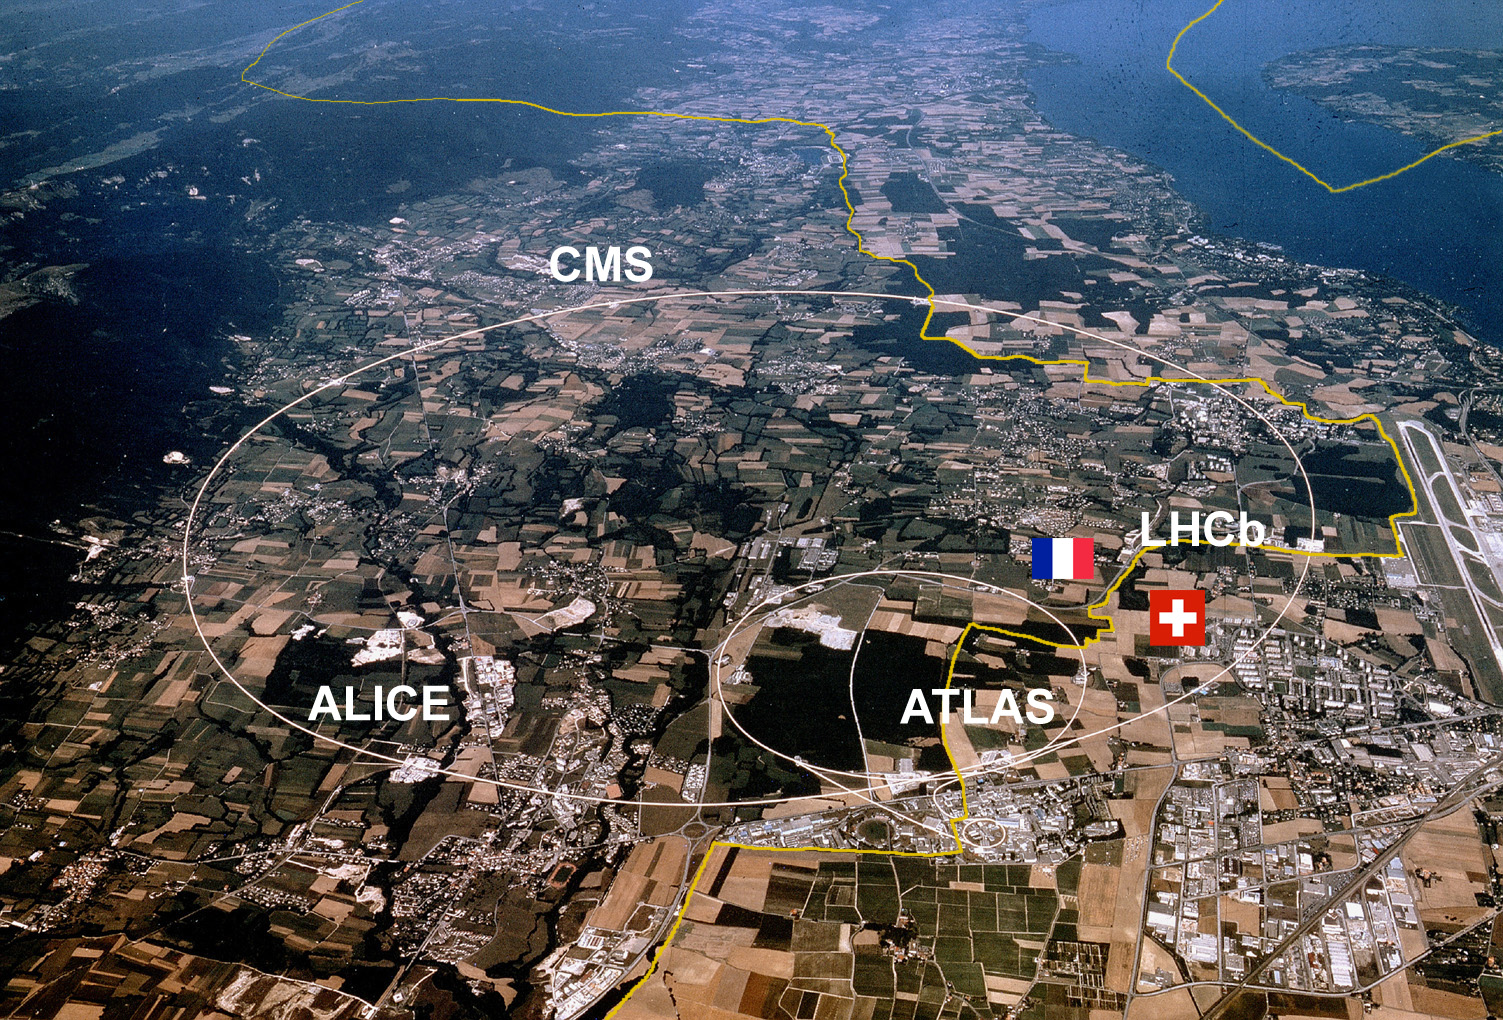
\includegraphics[width=\textwidth]{figs/lhc.jpg}
  \caption{The approximate location of the LHC ring traced over the Swiss-French border near Geneva, Switzerland. Also indicated are the relative locations of the two high luminosity experiments (CMS and ATLAS), the low luminosity B-physics dedicated experiment (LHCb), and the dedicated ion experiment (ALICE).}
  \label{fig:LHC}
\end{figure}

The total center-of-mass energy of a beam collision is the sum of the energy of the two incoming beam~\cite{martin2008particle}, and the LHC is designed to reach a center-of-mass collision energy of up to $\sqrt{s}=14\:\TeV$, with each beam able to reach energies of $7\:\TeV$. The total number of events that are generated in an LHC collision are given by $N_{\textrm{event}}=L\sigma_{\textrm{event}}$, with $\sigma_{\textrm{event}}$ being the cross section for the relevant measured event and $L$ being the machine luminosity. $L$ depends only on the beam parameters and goes as,

\begin{equation}
  L = \frac{N_{\textrm{b}}^{2}n_{\textrm{b}}f_{\textrm{rev}}\gamma_{\textrm{r}}}{4\pi\epsilon_n\beta^*}F,
  \label{eq:lumi}
\end{equation}

where $N_{\textrm{b}}$ is the number of particles per bunch, $n_{\textrm{b}}$ is the number of bunches per beam, $f_{\textrm{rev}}$ is the revolution frequency, $\gamma_{\textrm{r}}$ is the relativistic gamma factor, $\epsilon_n$ is the normalized transverse beam emittance, $\beta^*$ is the beta function at the interaction point (IP), and $F$ is the geometric luminosity reduction factor due to the crossing angle at the IP. The peak LHC design luminosity $L=10^{34}\:\textrm{cm}^{-2}\:\textrm{s}^{-1}$ dictates the necessity of high beam intensities, thus proton rather than anti-proton beams are used. The two beams of equally charged particles are circulated in opposite directions within separate beam pipes, and accelerated using separate and opposite magnet dipole fields and vacuum chambers in the main arcs.

The point of commencement for the protons circulated in the main LHC ring is a bottle of hydrogen gas at one end of the Linear accelerator 2 (Linac 2). Passing through an electric field that strips the hydrogen of its electrons, the remaining protons enter the Linac 2 and pass through alternating positive and negative cylindical conductors charged by radiofrequency cavities, which push and pull the protons causing them to accelerate to approximately $50\:\MeV$. The protons then enter the Proton Synchrotron (PS) Booster, which accelerate the beams to $1.4\:\GeV$ by means of four superimposed synchrotron rings. The protons then enter the PS, which is 628 m in circumference and accelerates the beams to $25\:\GeV$ through the use of conventional (i.e. not superconducting) magnets, of which 100 are dipoles that bend the beams around the ring. At this stage, a package of roughly one hundred billion protons, known as a ``bunch'', is separated from another bunch by a spacing of 25 ns, meaning that a proton bunch now rotates at 40 MHz. The following stage is the Super Proton Synchrotron (SPS), which has the same function as the PS, however with a circumference of nearly 7 km and 744 dipole magnets, the SPS is able to accelerate the proton beams up to an energy of $450\:\GeV$. At this stage the proton beam undergoes a bifurcation into bunch trains with two beams which enter the LHC moving in opposite directions. The chain is illustrated in~\FigureRef{fig:accelerator} showing an overview of the CERN accelerator complex and the aforementioned experiment IPs.

\begin{figure}
  \centering
  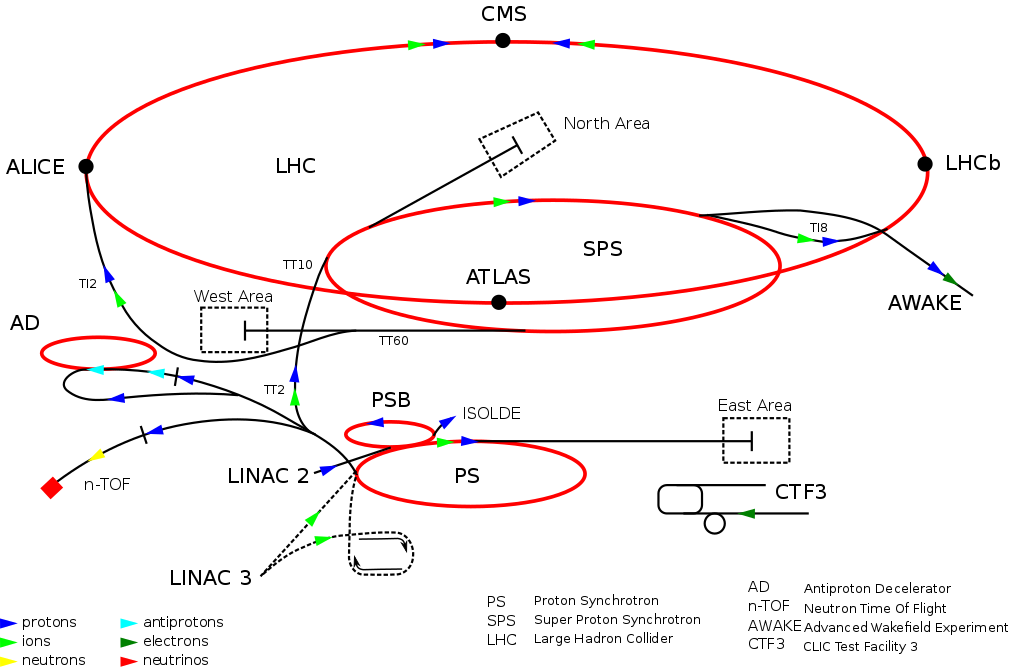
\includegraphics[width=\textwidth]{figs/accelerator.png}
  \caption{A schematic of the CERN accelerator complex, where protons (blue arrows) and ions (lime green arrows) begin their journey to the main LHC ring at the Linac 2 and Linac 3, respectively.}
  \label{fig:accelerator}
\end{figure}

Once injected into the LHC, the proton beams undergo a ramp up in energy in order to reach the maximum design energy of $7\:\TeV$ per beam, typically making $10^5$ traversals of the ring. In order to achieve these energies, the beam traverses a number of radiofrequency cavities, which are cooled with liquid helium to an operating temperature of 4.5 K. In addition, 1232 superconducting dipole magnets measuring 15 m in length are used to constrain the beam in a near circular path with a generated magnetic field of approximately 8.33 T, whilst 392 quadrupole magnets supercooled to 1.9 K and measuring 5-7 m, focus the beams and facilitate the collisions at the designated IPs. Between 2010-2011 and during 2012, the LHC collided proton beams at $\sqrt{s}=7\:\TeV$ and $\sqrt{s}=8\:\TeV$ respectively, while the energy increased to $\sqrt{s}=13\:\TeV$ in 2015 and 2016. The peak instantaneous stable luminosity reached by the LHC during 2016 was $1.527\times 10^34\:\text{cm}^{-2}\:\text{s}^{-1}$ and the total integrated luminosity delivered by the machine as a function of time can be seen in~\FigureRef{fig:LHClumi}, where the performance of the LHC was better than projected for 2016.

\begin{figure}
  \centering
  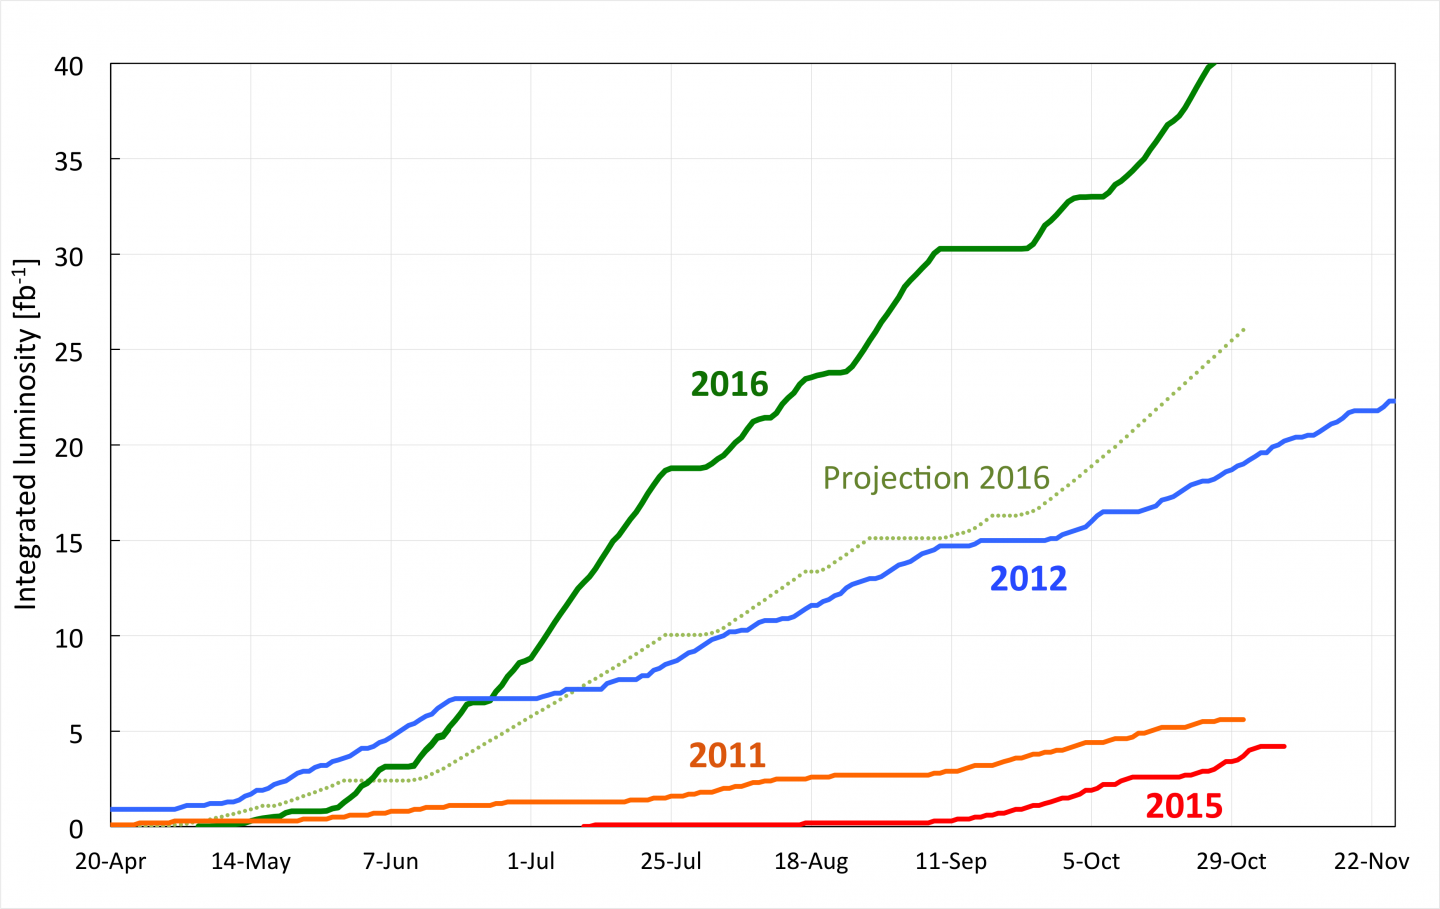
\includegraphics[width=\textwidth]{figs/lumi-proj-2016-final-v2.png}
  \caption{The integrated luminosity as a function of time that the LHC delivered at $\sqrt{s}=7\:\TeV$ and $\sqrt{s}=8\:\TeV$ during 2011 and 2012, and at $\sqrt{s}=13\:\TeV$ during 2015 and 2016.}
  \label{fig:LHClumi}
\end{figure}

\section{The \CMS experiment}
\label{sec:CMSInDetail}

Quantities described in this and following sections and chapters will rely heavily on the cylindrical coordinate system defined by the detector structure. The $z$-axis is defined to be parallel to the beam pipe pointing in the direction towards the Jura mountains from IP5, the azimuthal angle $\phi$ is defined in the transverse $x$-$y$ plane perpendicular to the beam line, and $\theta$ is the polar angle measured from the $z$-axis, as shown in~\FigureRef{fig:coordinates}. Consequently, quantities such as \pt, the transverse momentum, and \Et, the transverse energy are defined in terms of the respective momentum and energy in the $x$-$y$ plane. Rather than using $\theta$ to describe the direction of a particle trajectory within the detector, it is common practice in the case of highly relativistic particles to use $pseudorapidity$ defined as, 

\begin{equation}
  \eta = -\ln{\Big[\tan\big(\frac{\theta}{2}\big)\Big]} = \frac{1}{2}\ln{\Big(\frac{|\textbf{p}|+p_{z}}{|\textbf{p}|-p_{z}}\Big)} 
\end{equation}

in terms of both the polar angle, and $\textbf{p}$, the three momentum and $p_{z}$, the momentum along the $z$-axis. $\eta=0$ for $\theta=90^\circ$ and approaches infinity as the polar angle goes to 0. $\eta$ regions in detector are often referred to as ``barrel'' denoting the central $|\eta|$ region from 0 to $\approx 1.2-1.6$, ``endcap'' denoting the region up to $|\eta|\approx 3$, and ``forward'' denoting the region beyond the endcap. The definitions are subject to slight differences depending on the reconstruction of the object in question.

\begin{figure}
  \centering
  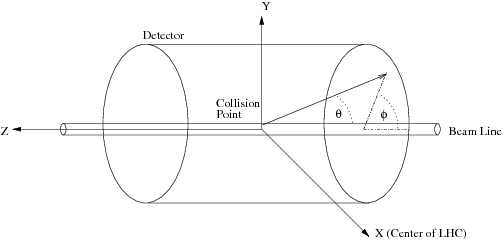
\includegraphics[width=0.7\textwidth]{figs/Figures_T_Coordinate.png}
  \caption{A diagram of the cylindrical coordinate system for the CMS detector.}
  \label{fig:coordinates}
\end{figure}

The CMS detector, described in detail in~\cite{Chatrchyan:2008aa}, is a multi-purpose apparatus designed to study high-\pt physics processes in proton-proton and heavy-ion collisions. In 2016, CMS collected approximately $37.8\:\textrm{fb}^{-1}$ of integrated luminosity as seen in~\FigureRef{fig:CMSlumi}, of which $35.9\:\textrm{fb}^{-1}$ were certified as usable for physics analysis. The CMS detector relies on a superconducting solenoid magnet located in its central region to provide a magnetic field of 3.8 T parallel to the beam direction. Charged particle trajectories are measured by silicon pixel and strip trackers, which cover a pseudorapidity region of $|\eta| < 2.5$. Surrounding the tracker volume are a lead-tungstate crystal electromagnetic calorimeter (ECAL) and a brass-and-scintillator hadron calorimeter (HCAL) surround the tracking volume, covering the region of $|\eta| < 3$. A steel and quartz-fiber Cherenkov forward hadron calorimeter extends the coverage to $|\eta| < 5$. The muon system consists of gas-ionization detectors embedded in the steel flux return yoke outside the solenoid, and covers the region with $|\eta| < 2.4$. The detector is designed to cover a 4$\pi$ solid angle as illustrated in~\FigureRef{fig:CMSCrossSection}, demonstrating the overall scale of the experiment and the surrounding cavern structure.

\begin{figure}
  \centering
  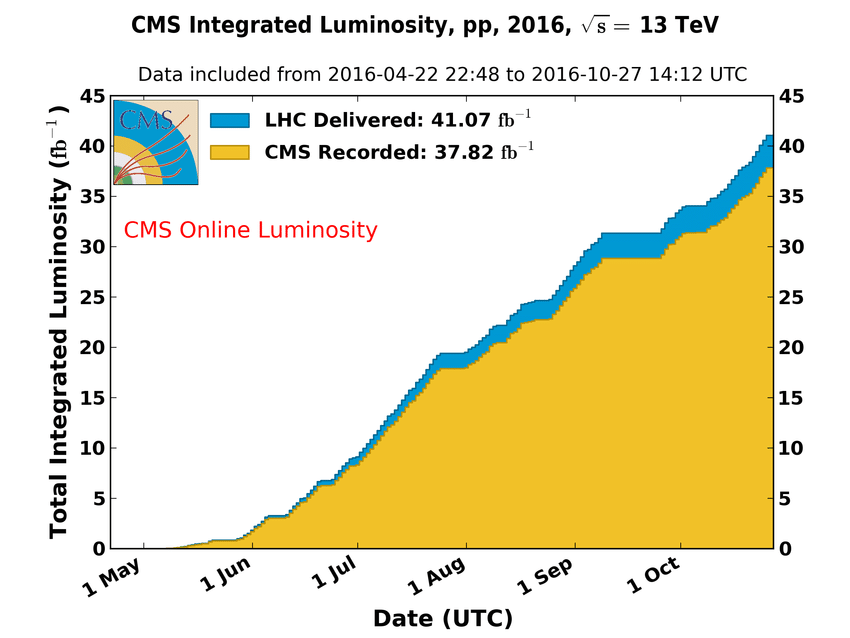
\includegraphics[width=\textwidth]{figs/CMSLUMI.png}
  \caption{The total integrated luminosity that the LHC machine delivered to CMS, and the total integrated luminosity that the detector collected during the 2016 data-taking period~\cite{CMSLumi}.}
  \label{fig:CMSlumi}
\end{figure}

\begin{sidewaysfigure}
  \centering
  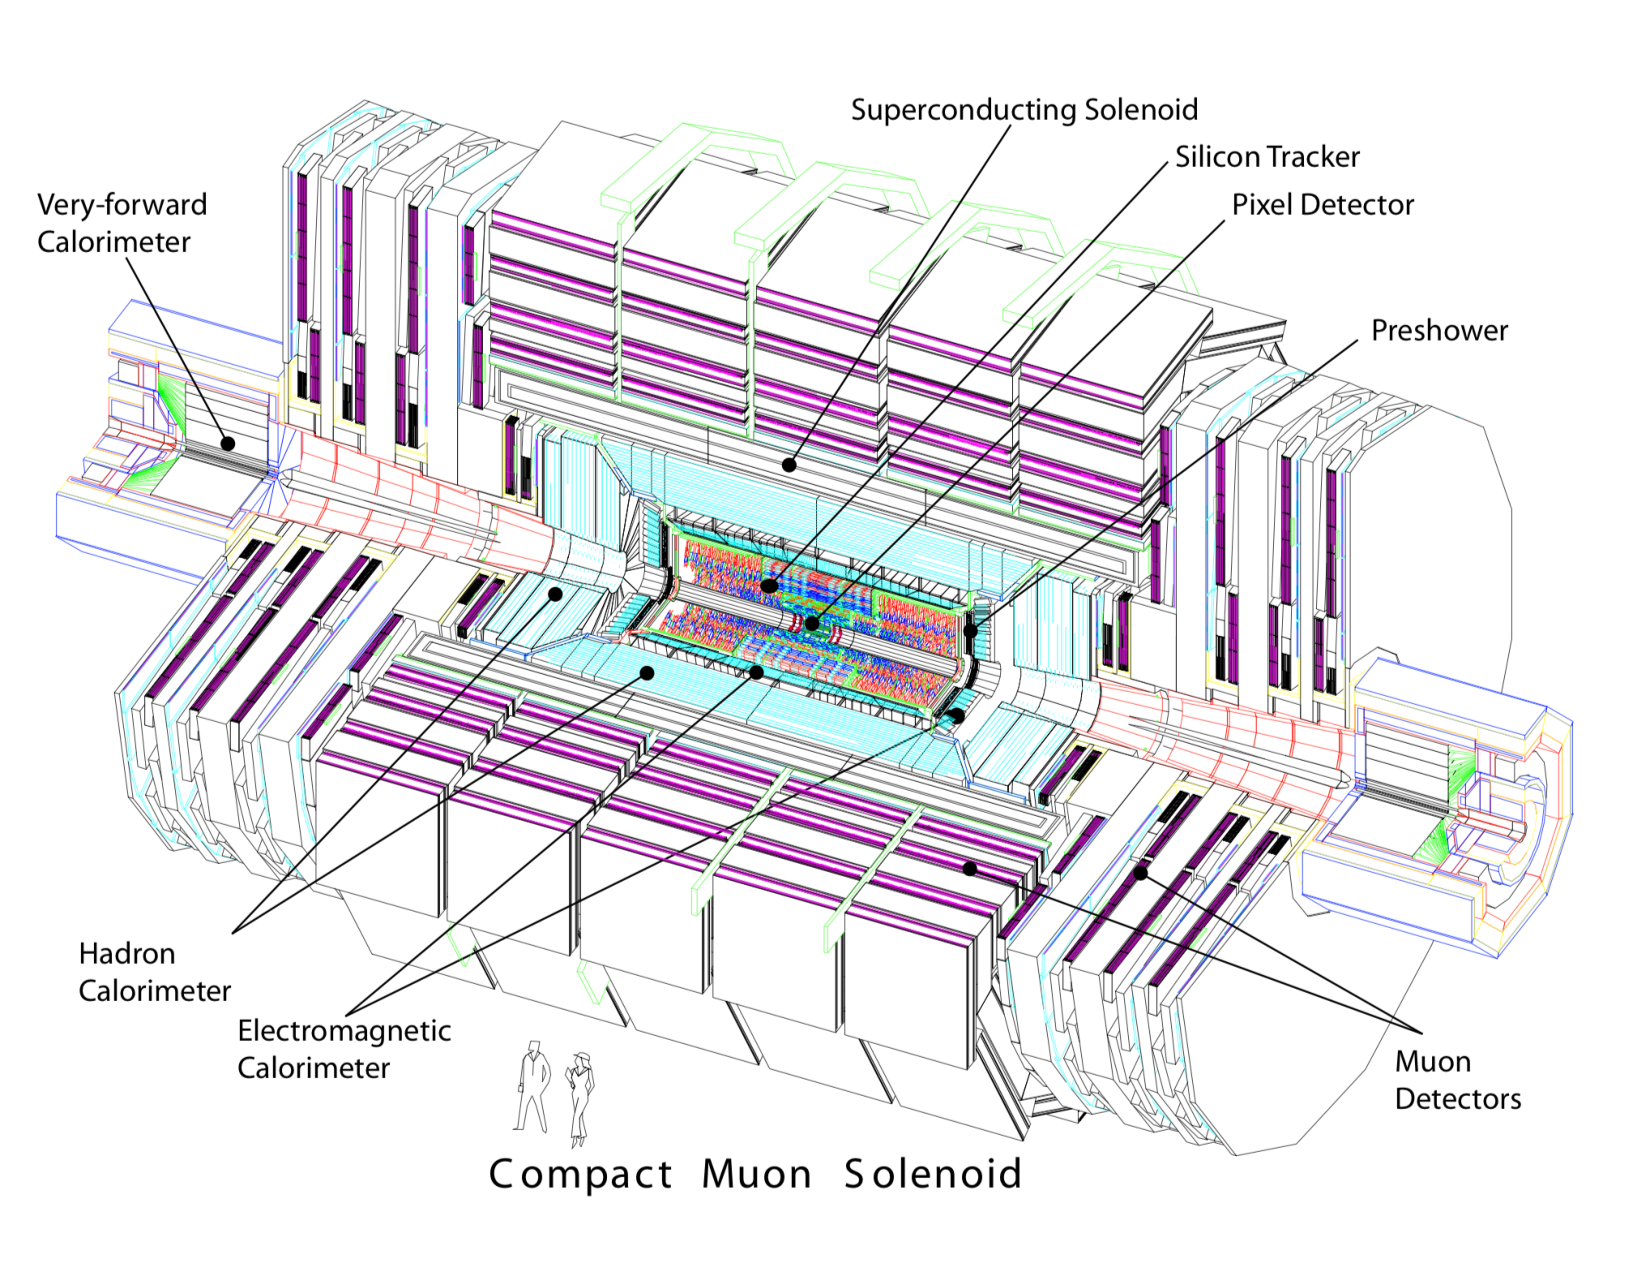
\includegraphics[width=0.8\textheight]{figs/CMScrosssection.pdf}
  \caption{Cross-section view of \CMS~\cite{Chatrchyan:2008aa}.}
  \label{fig:CMSCrossSection}
\end{sidewaysfigure}

\subsection{The magnet}
\label{subsec:magnet}

The benefit of the strong magnetic field provided by the superconducting solenoid is the improvement in the momentum resolution for muons, and the increase efficiency of the inner tracking~\cite{tdrmagnet}. The main components comprising the magnet are the superconducting solenoid coil, the 1.5 m thick saturated iron yoke in the barrel and endcap regions which return a 2 T magnetic flux, vacuum chambers, and the cryogenic system. Stabilised, reinforced NbTi conductor is used for the 4-layer winding of the coil cold mass, which measures 12.5 m in length. Since the CMS magnet can achieve a stored energy and an energy-to-mass ($E/M$) ratio significantly larger than any other previous detector magnet technologies, the shear stress level inside the coil winding is non-negligible, thus an innovative self-supporting aluminum conductor is included in the magnet structural material to mitigate these effects. 

The 3.8 T field that is generated inside the solenoid bends charged particle trajectories in the enclosed silicon tracking detector, enabling the measurement of the \pt of a particle track via the azimuthal angle $\phi$, which is related to the bending radius $\rho$ and the magnet length $L'$ by $\phi = L'/\rho$. Thus measuring the $\rho$ of a charged particle track, 

\begin{equation}
  \pt \propto z\rho B,
\end{equation} 

where $B$ is the magnetic field in the $z$ direction, parallel to the beam axis, and a particle charge of $ze$ is assumed. The muon system stations, described in greater detail in \SectionRef{subsec:muons} interleaved in the iron yoke are also subjected to a 2 T return flux, causing charged particles to bend in the opposite direction from their trajectory within the inner tracker volume. Multiple measurements $N$ made along the trajectory of a uniform medium provide the curvature ($k=1/\rho$) error $\delta k_{\textrm{res}}$ due to finite measurement resolution which goes as,

\begin{equation}
  \delta k_{\textrm{res}} = \frac{\epsilon}{L'}\sqrt{\frac{720}{N+4}}
\end{equation} 

\subsection{The inner tracker}
\label{subsec:tracker}

\begin{figure}
  \centering
  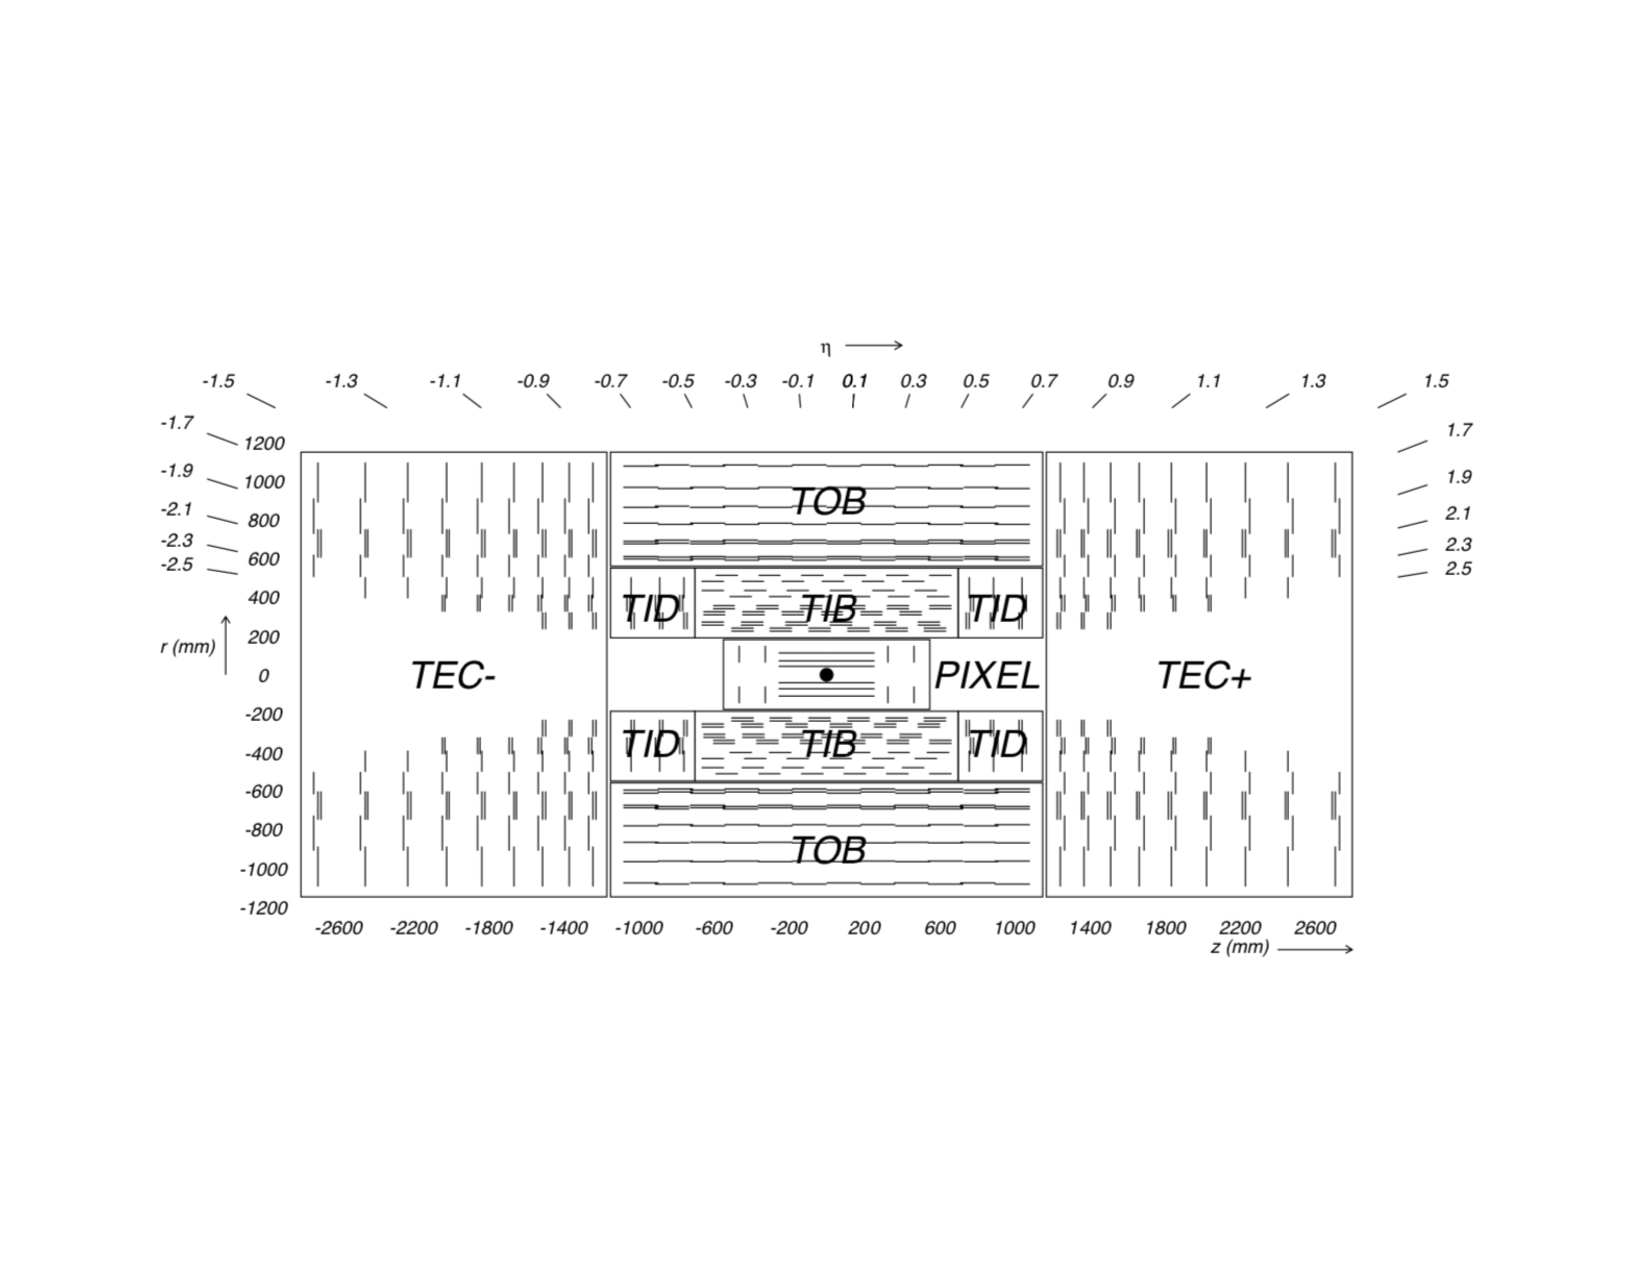
\includegraphics[width=\textwidth]{figs/tracker_schematic.pdf}
  \caption{Schematic cross-section through the \CMS tracker, where a single detector modules is represented by a line, and double lines signify back-to-back modules~\cite{CMS:1998aa}.}
  \label{fig:trackerxsec}
\end{figure}

One of the main mandates of the CMS detector is to provide good resolution and reconstruction efficiency for charged particles emmitted from LHC collisions in the inner tracker, of which a cross-sectional view is shown in~\FigureRef{fig:trackerxsec}. Furthermore, the precise reconstruction of secondary vertices is imperative for the efficient identification of b-jets; b-jets are heavily employed in the as a effective handles in the identification of a \ttll final state topology. To achieve this, it is imperative for the positioning of tracker layers to be close to the interaction point of a collision, hence the three pixel barrel (BPix) layers are stationed at radii 4.4 cm, 7.3 cm, and 10.4 cm from the interaction point. Designed to keep the occupancy of these inner layers below $1\%$, the silicon pixel cells measure 100 x 150 $\mum^2$ in $r-\phi$ and $z$ respectively, of which 52 x 80 cells populate one read-out chip (ROC) and 16 ROCs comprise one BPix module sensor. In order to cover out to $|\eta|<2.5$, the pixel detector also has two endcap disks (FPix) stationed on either side of the BPix at $z=\pm34.5$ and $z=\pm46.5$ cm and extending from 6 to 15 cm in r. The FPix consists of varying trapezoidal (pie-shaped) panels which contain different numbers of $plaquettes$ consisting of single pixel sensors bump-bonded to a varying number of ROCs. The sensors are offset on the panels so as to ensure there are no cracks in the endcap $\eta$ coverage. The BPix and FPix deliver up to three high precision spatial point positions (hits) for which the resolution in $r-\phi$ is up to 10 \mum and that in $z$ is up to 20 \mum. The operating temperature of the pixel detector during 2016 was $-10^\circ$C.

Surrounding the pixel layers are the four and six silicon strip layers comprising the Tracker Inner Barrel (TIB) and Tracker Outer Barrel (TOB), respectively. The TIB extends radially from 20 to 55 cm, with a relative occupancy of $2-3\%$ per strip module in this intermediate region. The distance between the p+ type strip implants in the n type $\textrm{SiO}_{2}$ bulk of the strip sensors is called the pitch~\cite{Borrello:2003uza} and is approximately 80 \mum for the first two layers and 120 \mum for the third and fourth TIB layers, providing a hit resolution of 23 \mum and 35 \mum respectively. The TOB covers a region out to $|z|<118$ cm along the beampipe and makes use of thicker (500 \mum) strip sensors as compared to those used for the TID (320 \mum) in order to maintain a signal-to-noise ratio greater than 10. The first four layers of the TOB make use of strips with a pitch of 183 \mum, while the strip pitch in layers 5 and 6 is 122 \mum, providing hit resolutions ranging from 53 \mum to 35 \mum. The strip hit resolutions in the TIB and TOB for 2016 are summarized in~\FigureRef{fig:striphitres}. The last TOB layer reaches an outward radius of 110 cm from the beampipe. The TIB and TOB are complimented by disk layers on both $\pm z$ sides, with the Tracker Inner Disks (TID) consisting of three small disks flanking the TIB and the Tracker EndCaps (TEC) consisting nine larger disks flanking the TOB. The pitch for the 320 \mum thick micro-strip detectors employed in the TID varies from 100 \mum to 141 \mum. The TEC has a positive (TEC+) and negative (TEC-) $z$ side, where the nine disks on either side extend from $124 < |z| < 282$ cm and radially from $22.5 < |r| < 113.5$ cm. The disks can have up to seven rings, of which the four innermost are comprised of 320 \mum thick micro strip sensors while the fifth through seventh are 500 \mum in thickness. A maximum of nine $\phi$ hit measurements can be obtained from each TEC disk. In addition, the innermost two layers of the TIB and TOB, and the innermost two disks TID consist of double-sided strip modules. The same is true for the first, second and fifth wheel of the TEC+/- disks. For such modules, the second module is mounted back-to-back at a stereo angle of 100 mrad in order to make it possible to compute a 2D position measurement, by also providing the $z$ coordinate in the barrel and $r$ coordinate on the disks, along with the $\phi$.

The layout of the inner tracker guarantees approximately nine hit measurements up to $|\eta| < 2.4$, at least 4 of which are 2D measurements. The performance of the tracker is gauged by the resolutions for the \pt, the transverse impact parameter ($\textrm{d}_0$), and the longitudinal impact parameter ($\textrm{z}_0$) expected for single muons of varying \pt. In the case of single muons with a \pt equal to 10 and 100 \GeV, (i.e. the range considered in the following work), the \pt resolution is 0.65$\%$ and 1.5$\%$ respectively at $\eta=0$, and reaches $1\%$ and $2\%$ for $|\eta|=1.6$.

\begin{figure}
  \centering
  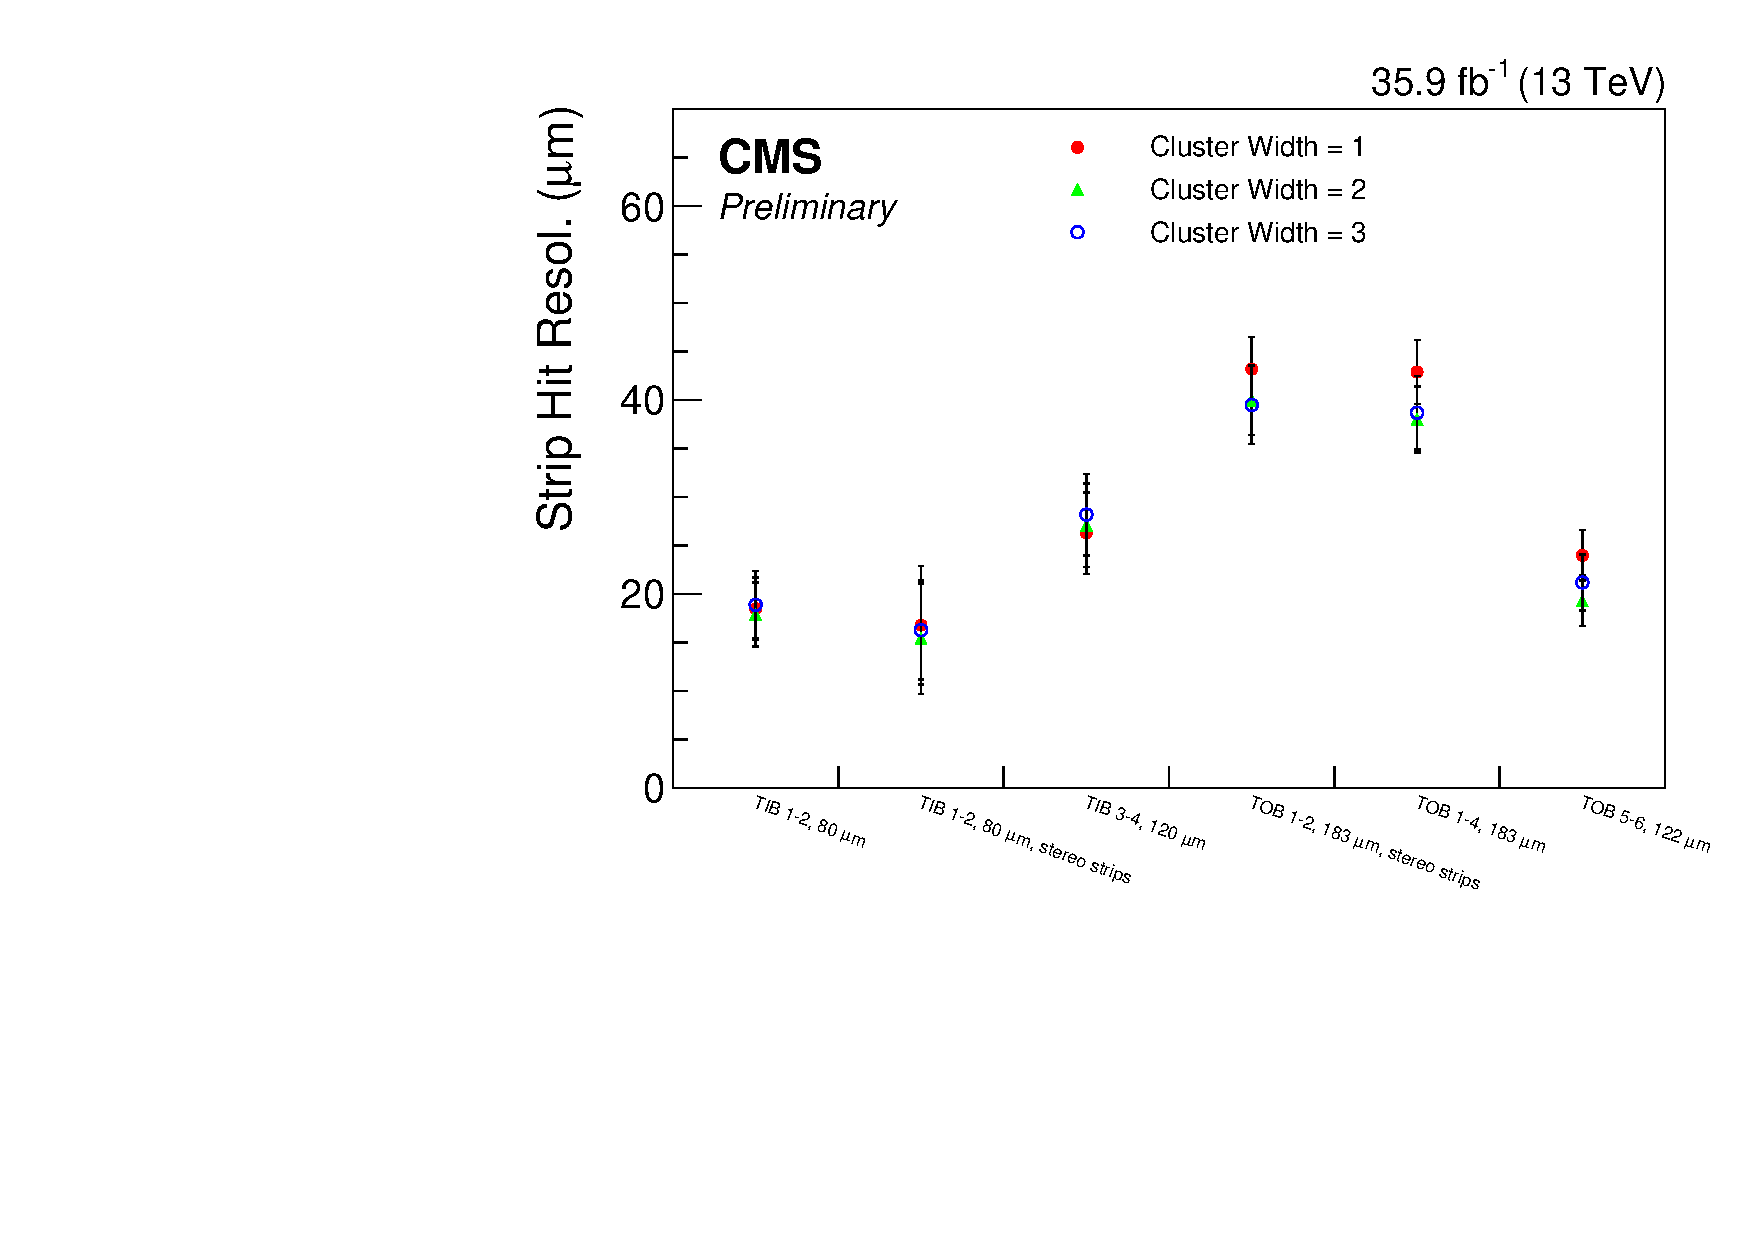
\includegraphics[width=0.7\textwidth]{figs/StripHitRes.pdf}
  \caption{The strip hit resolution for the TIB and TOB layers which are comprised of Si sensors with varying strip pitch. The tracks selected have $\pt>3\:\GeV$, at least six hits in the inner tracker, and $\chi^2$ probability greater than nine~\cite{TRKDPG}.}
  \label{fig:striphitres}
\end{figure} 

\subsection{The calorimeters}
\label{subsec:calos}

Along with tracking information, in order to measure electron \pt and energy, a calorimeter system is of utmost importance. Other mandates of the calorimetry system include the measurement of hadronic jet energies and the inference of the existence of neutral particles within the detector volume such as $\pi^{0}$s or photons (\gamma). The CMS calorimeter system is comprised of an electromagnetic calorimeter and a brass and scintillating hadronic calorimeter. 

\subsubsection{The ECAL}
\label{subsubsec:ECAL}

The ECAL is a hermetic and homogeneous calorimeter which consists of a barrel (EB) region, from $0 < |\eta| < 1.48$, and two endcap regions (EE), from $1.48 < |\eta| < 3.0$. Chosen for its short radiation length ($X_0$) and correspondingly small $\textrm{Moli}\grave{\textrm{e}}\textrm{re}$ radius ($R_{M}$), the ECAL is comprised entirely of lead tungstate crystals ($\textrm{PbWO}_4$). The two quantities are related by, 

\begin{equation}
  R_{M} = 0.0265X_{0}(Z+1.2),
\end{equation}

where $Z$ is the atomic number. With the ability to emit $80\%$ of the scintillating light within 25 ns, the crystals are fast light emitters with an emission peak located at 425 nm allowing for a suitable combination with photo-detectors~\cite{Cockerill:2008td}. With $X_0 = 0.89$ cm and $R_M=2.2$ cm, a better electromagentic (EM) shower position and shower separation is achieveable because of the compact nature and fine granularity of the detector. The EB crystals are approximately 25.8$X_0$ (23 cm) in length and cover an area of 2.6x2.6 cm$^2$ at the rear, while the EE crystals are 24.7$X_0$ (22 cm) in length and cover an area of 3x3 cm$^2$ at the rear. In dimensions of $\Delta\eta$x$\Delta\phi$, the area that is subtended by a crystal in the EB is 0.0175x0.0175, while the area varies from 0.0175x0.0175 to 0.05x0.05 for the EE crystals. The scintillation light is detected by the use of avalanche photodiodes (APDs) in the EB, with a total of two APDs glued to each crystal. Both the APDs, which operate at a gain of 50, and the crystal scintillation have a temperature dependence of approximately $-2.4\%/^{\circ}$C, which dictates the operation of the ECAL to within $\pm0.05^{\circ}$C. Vacuum photo-triodes (VPTs) are employed in the EE because of their increased radiation resistance compared to the silicon diodes. 

In front of each EE, flanking the inner tracker TEC+/- disks sits a preshower detector covering $1.65<|\eta|<2.6$ which consists of 2$X_0$ and 1$X_0$ depth of lead absorber strips, behind which are two orthogonal planes of silicon strip detector. The preshower aids in the discrimination between $\pi^0\rightarrow\gamma\gamma$ process and Higgs decays of $h\rightarrow\gamma\gamma$, since the relatively short lifetime of the $\pi^0$ results in its decay to a diphoton pair upstream of the ECAL where photon conversion in the lead absorber may result. The $\gamma\rightarrow e^+e^-$ conversions will leave hits in the silicon strips beyond the absorber along with an energy deposit in the ECAL crystals.

The energy resolution of the ECAL contains three contributions: a stochastic term, a noise term, and a constant term listed in order in the following~\cite{Chatrchyan:2013dga},

\begin{equation}
 \frac{\sigma_{E}}{E} = \frac{2.8\%}{\sqrt{E}} \oplus \frac{12\%}{E} \oplus 0.3\%,
\end{equation}

where the EB energy resolution is obtained using electrons incident on 5x5 arrays of crystals, and the EM showers are reconstructed in a 3x3 matrix of crystals inside the array around the electron impact point. 

\subsubsection{The HCAL}
\label{subsubsec:HCAL}

\begin{figure}
  \centering
  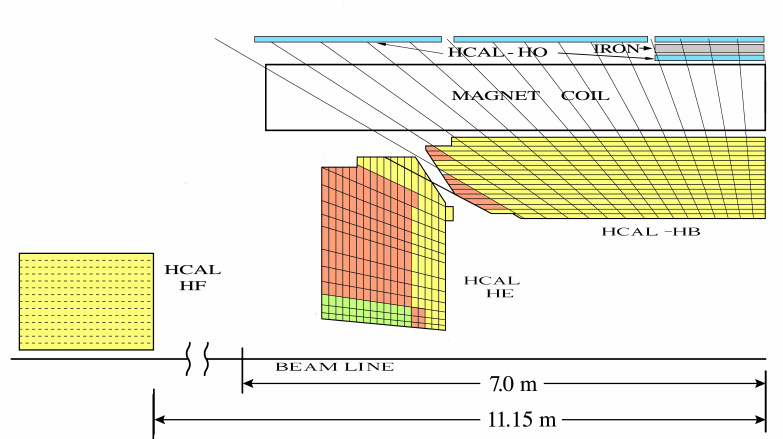
\includegraphics[width=0.8\textwidth]{figs/quarterHCAL}
  \caption{A quarter-view of the CMS hadron calorimeter. The shading indicates the grouping of scintillating layers optically added together to form trigger tower signal readouts.~\cite{Chatrchyan:2009hy}}
  \label{fig:hcal}
\end{figure}

The hadron calorimeter (HCAL), of which a quarter-view is shown in~\FigureRef{fig:hcal}, is essential to the measurement of the energy and direction of particle jets. In conjunction with the ECAL and the muon system, the HCAL also aids in the identificaition of electrons, photons and muons. Hadronic calorimetry is in general considered to be more challenging than the EM calorimetry discussed in the above section, in part due to the much larger depth of detector material required to contain a hadronic cascade in comparison to the EM fraction emmitted in the ECAL. Furthermore, the energy resolution of the HCAL is worsened compared to that of the ECAL by so-called intrinstic fluctuations, which are a result of the significant incoming energy fraction being invisible, since it is employed in processes like nuclear break-up~\cite{Leroy:2004zza}. 

Located inside the solenoid magnet cryostat, the CMS HCAL consists of four distinctive regions, where the barrel (HB) covers the $|\eta|$ range from 0 to 1.4, while the endcap (HE) covers the $|\eta|$ range from 1.3 to 3.0, thus the HB and HE share the $|\eta|$ range from 1.3 to 1.4. The calorimeter is based on sampling detector technology, and both the HB and HE consist of brass (copper) absorber plates interleaved with plastic scintillator where the sampling fraction is approximately 7$\%$. The HB consists of 18 wedges, where each covers $20^\circ$ in $\phi$ and this area is further divided into $5^\circ$ sectors. The composition and segmentation of the HE is similar, and extends from 388 cm < $|z|$ < 5.68 cm on either $\pm z$ side. The space constraint from the magnet cryostat at $\eta=0$ requires the HB thickness be limited to approximately 5.8 nuclear interaction lengths ($\lambda_{I}$) and increases to 10$\lambda_{I}$ at $|\eta|=1.2$. The nuclear interaction length is the mean free path that an incident hadron can travel in a medium before the nuclear interaction resulting in the absorption of the hadron occurs, and is a material constant that goes as, 

\begin{equation}
  \frac{1}{\lambda_{I}} = \sigma_{\textrm{inel}}\cdot\frac{N_A\cdot\rho}{A}
\end{equation}

where $\sigma_{\textrm{inel}}$ is the inelastic cross-section, $\rho$ is the density, and $A$ is the atomic mass of the absorber. At 10$\lambda_{I}$, more than 99$\%$ of the hadronic cascade is contained within the detector material. In the HB and HE, the scintillation light that is captured is then wavelength shifted, and guided to hybrid photodiodes (HPDs).

In addition to the HB and HE, the main objectives of the forward part of the HCAL (HF) involve the improved measurement of the missing transverse energy and to ensure the identification and reconstruction of very forward jets. The HF covers the $|\eta|$ region from 3.0 to 5.0, and the front face is located at $|z|$=11.1 m from the IP. Due to the high operational luminosity of the LHC and subsequently high average particle multiplicity at the IP per bunch crossing, the inner part of the HF ($4.5 < |\eta| < 5$) is subjected to the largest particle flux, which when absorbed by the detector can reach radiation doses close to 100 Mrad/year. As a result, the HF is constructed with the capability to survive in a high radiation field, hence the absorber is iron and embedded with dual-length quartz fibres parallel to the beam pipe. The HF is segmented into 20$^\circ$ wedges in $\phi$ where each wedge contains two $10^\circ\:\phi$ sectors. The particles that enter the absorber subsequently produce a shower of particles and those traversing the quartz fibres produce Cherenkov light in the fibres which is guided to the photomultipliers (PMTs). In order to distinguish between showers emmitted from e/$\gamma$ and hadrons, short and long fibres of approximately 165 cm and 22 cm, respectively, are used where the typical electromagnetic shower is known to be shorter and more collimated than charged hadron showering.

The final part of the HCAL, located outside the solenoid cryostat, is the outer HCAL (HO) which consists of layers of scintillators and serves to catch any energy leakage from the HB. Approximately $5\%$ of particles with $\pt > 100\:\GeV$ deposit some energy fraction in the HO, since complete containment of the hadronic shower in the $0 < |\eta| < 1.4$ is not feasible.

\subsection{The muon detectors}
\label{subsec:muons}

The CMS muon system is used as an exceptionally powerful tool for recognizing interesting physics processes over high background rates, and has a three-fold objective: triggering, identification, and precise momentum measurement. In particular, the latter objective is achieved as a result of the high spatial resolution of the detector and the high magnetic field of the solenoid coil and the flux-return yoke. The CMS muon spectrometer is designed to measure the momentum and charge of muons over a large kinematic range, and operate in high flux regions with non-uniform magnetic field strengths.

Comprised of both a barrel and endcaps, the muon system is situated outside of the magnet solenoid and is interleaved with layers of the steel flux-return yoke. The technologies used in both the barrel and endcaps are three types of gas ionization particle detectors and in all cases throughout the following section, the physical modules are referred to as ``chambers''. Since the magnetic field is diminished to approximately 2 T outside of the solenoid magnet and subsequently reverses the muon trajectory, recording several muon track measurements along the trajectory is necessary for the momentum calculation. For this reason, the drift tube (DTs) chambers used in the barrel are positioned along several values of $r$ in the radial direction and the cathode strip chambers (CSCs) used in the endcaps are positioned along several values of $z$ parallel to the beampipe, as shown in~\FigureRef{fig:muondet}. There are four stations in the barrel labeled MB1-MB4, and four stations in each of the endcaps labeled ME1-ME4, where a station is an assembly of chambers.

Owing to the low muon rate, along with low neutron background rate expected in the barrel region, and the relatively uniform and weak magentic field inside the chambers (0.4 T), DTs are employed in this region. Each DT chamber consists of many drift cells, each filled with $85\%/15\%$ Ar/CO$_2$ and having two cathode strips on either side, and electrodes on the top and bottom walls of the cell. A singular 50 \mum gold-plaited anode wire operating at +3.6 kV is centrally located within the cell volume. Meanwhile the cathodes are operated at -1.8 and +1.8 kV respectively, thus if a muon is incident on the DT, the electrons released in the gas volume drift to the anode and produce avalanches in the increasing field inside the cell. A DT chamber is comprised of three superlayers, where one is placed orthogonally to the remaining two so as to obtain both an $r-\phi$ and $r-z$ position measurement. A superlayer consists of four staggered layers of cells.

Conversely to the barrel case, both the muon rate and the neutron background rate are much higher in the endcaps, thus CSCs are used for their fast response time, owing to the short drift path. The endcaps are also subjected to a higher and non-uniform magnetic field and the CSCs, unlike the DTs, can tolerate this environment. Another benefit to the use of CSCs is their ability to be finely segmented providing a increased momentum resolution. Covering an $|\eta|$ region of 0.9 to 2.4, there are four stations of chambers mounted onto the faces of steel disks perpendicular to the beam line, and each chamber consists of 6 layers of CSCs with cathode strips running radially out, while the 50 \mum diameter anode wires run perpendicularly to the strip orientation and are spaced out by 3.16 - 3.12 mm distances. Each station provides the muon position in $r-\phi$. The CSCs are multi-wire proportional counters with cathode strips which allow for the precise measurement of the position at which a muon or charged particle crosses the gas gap. The CSC stations are further divided into rings where n denotes the ring number and increases radially outward in the naming convention ME1/n-ME4/n. The innermost ring of the first station (ME1/1) is subdivided into two regions in order to allow for triggering and independent readout from the region closest to the beam line. 

In addition to the tracking detector technologies, the CMS muon detector also makes use of resistive plate chambers (RPCs) which are interspersed in the endcaps and barrel between the CSCs and DTs, respectively. Primarily used in fast and independent triggering over a range in $|\eta|$ up to 1.6, the RPCs consist of two gas gaps with readout strips aligned in \eta between the gas gaps. Charged particles traversing an RPC will ionize the gas in both volumes causing avalanches to generate as a result of the high electric field. The avalanches, in turn, induce an image charged which is caught by the readout strips. 

\begin{figure}
  \centering
  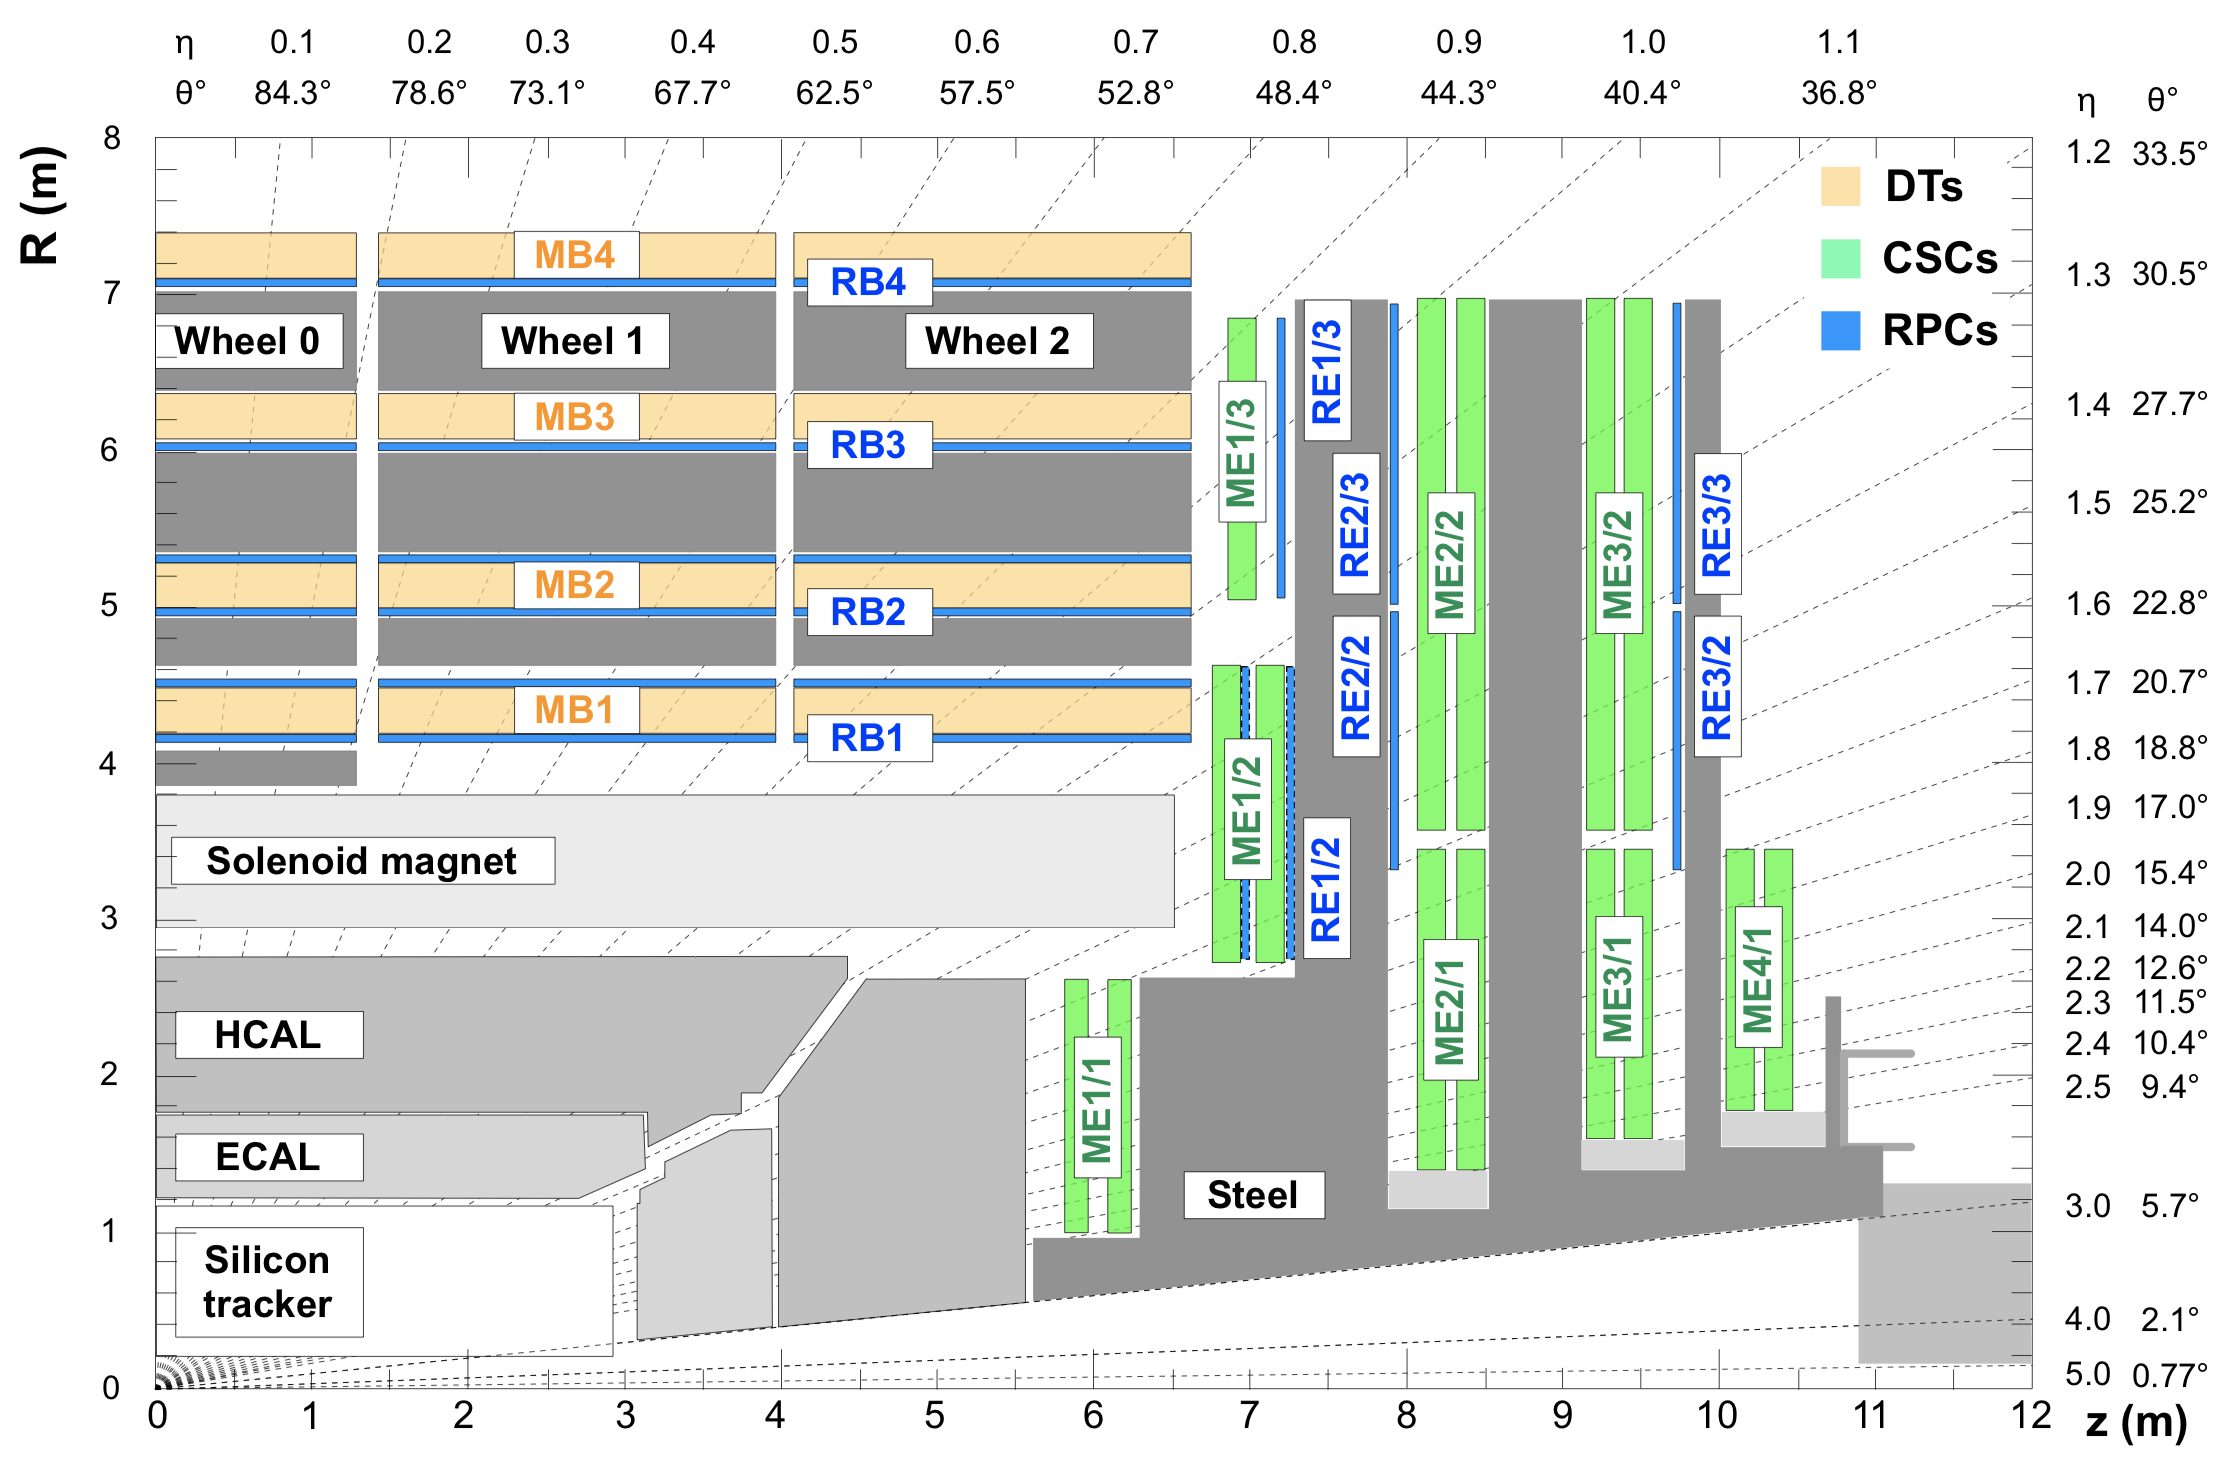
\includegraphics[width=0.8\textwidth]{figs/muonsys}
  \caption{A quadrant view of CMS where the IP is at the lower left corner. The dark grey areas denote the locations of the various muon stations and the steel disks. The 4 drift tube (DT, in light orange) stations are labeled MB (“muon barrel”) and the cathode strip chambers (CSC, in green) are labeled ME (“muon endcap”). The resistive plate chambers (RPC, in blue) located in the barrel and the endcaps of CMS, are labeled RB and RE, respectively.~\cite{Chatrchyan:2013sba}}
\label{fig:muondet}
\end{figure}

\subsection{The readout system}
\label{subsec:readout}

The 2016 run of the LHC delivered more than $6.5 \times 10^{15}$ collisions to each of the general purpose detectors. The time spacing of 25 ns between each collision corresponds to a beam crossing frequency rate of 40 MHz. In addition to this exceptionally high rate, on average 27 particle interactions per bunch crossing occured during the 2016 proton-proton run at $\sqrt{s}=13\:\TeV$ during which the LHC operated at unprecedented luminosities. In addition, the fine segmentation of the CMS subdetectors results in nearly 100 million readout channels and a correspondingly immense volume of data at the sub-detector front-end level. Hence, in order to maintain a high acceptance for events of interest, while simultaneously rejecting QCD multi-jet events which drive the readout rate to high values,  CMS employs a two-level robust triggering and detector readout system: a hardware-based Level-1 (L1) trigger which reduces the readout rate from 40 MHz to 100 kHz, and a software-based High-Level trigger (HLT) which further reduces the rate to approximately 200-300 Hz, before storing the data. The architecture of the triggering system can be seen in~\FigureRef{fig:trigger}.

\begin{figure}
  \centering
  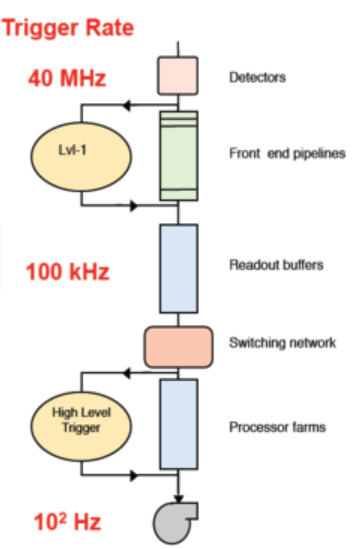
\includegraphics[width=0.3\textwidth]{figs/TriggerRate}
  \caption{A schematic of the two stage CMS trigger architecure and the corresponding rate reduction at each stage~\cite{Halyo:2013iba}.}
  \label{fig:trigger}
\end{figure}

The L1 CMS trigger system uses information from the previously described calorimeters and muon system to select the most interesting events in a fixed time interval of less that 4 $\mu$s, which allows for 1 $\mu$s of processing time.


The L1 triggering system relies heavily on the muon detector, where two independent and complementary technologies are employed. The DTs and CSCs in the barrel and endcaps respectively are tracking detectors which provide excellent position and time resolution, whereas the RPCs are used to correspondingly provide a very good timing resolution, but a cruder spatial resolution. For muons with \pt up to approximately $200\:\GeV$, the momentum resolution is largely dominated by multiple scattering in the steel flux-return yoke, especially in the endcaps, thus the multi-layer CSCs are exploited by the L1 trigger, in order to be able to achieve a high precision in constructing the track segments in the chambers. With the large number of layers and consequently track segments, sharp \pt trigger thresholds at L1 are achieved for muons with \pt up to approximately $100\:\GeV$.  The hits in the DTs and CSCs are used to construct track stubs at the chamber/sector level before they are forwarded to the designated sub-detector track-finders (DTTF and CSCTF). In order to guarantee the full coverage over the barrel-endcap transition region, these stubs are shared between the TFs. Correspondingly, the RPC uses hits in pattern comparator logic (RPC PAC) to identify potential muon candidates. The trigger primitives from these regional muon triggers are then forwarded to the Global Muon Trigger (GMT) where they are combined and the four best muon candidates in the barrel and endcap are forwarded to the Global Trigger (GT). 

In addition to the muon trigger, the ECAL and HCAL contribute to the calorimeter trigger. The ECAL detector is read out from groupings of 5x5 crystals, where the APDs or VPTs are connected to multi gain pre-amplifiers and these gain ranges are fed to an analog-to-digital converter (ADC) which digitizes the signal at 40 MHz. Energy deposits are calculated in barrel trigger towers, which are $0.0875\times 0.0875$ regions in $\eta-\phi$ space, and subsequently sent to the Regional Calorimeter Trigger (RCT). At this stage $e/\gamma$ candidates are identified and the energy is further summed into $0.35\eta\times 0.35\phi$ regions. This information is then passed to the Global Calorimeter Trigger (GCT) which performs the sorting of $e/\gamma$ candidates, identifies jets, and energy sums. The GCT then sends the GT four isolated and four non-isolated $e/\gamma$ candidates, and four jets of each category: forward, central, and tau. In addition, the GCT passes along total and missing energy sums (\Et and \MET), and scalar and magnitude of vector sums of transverse jet momenta ($H_\mathrm{T}$ and $MH_\mathrm{T}$)~\cite{Brooke:2013hnf}. A trigger menu is programmed at the GT level, which consists of approximately 128 trigger algorithms used to make specific requirements on the candidates that have been received from the GCT and GMT. Along with requirements on energy and \pt thresholds of these candidates, the GT is able to require combinations of objects and specify criteria having to do with their relative positions. The decision of whether to keep or discard data from a particular bunch crossing, known as a ``L1 accept'' is based on whether the trigger primitives, such as the electrons, muons, photons, and jets, pass the set \Et or \pt thresholds, and the total allocated time for the decision is 3.2 $\mu$s. 

\begin{figure}
  \centering
  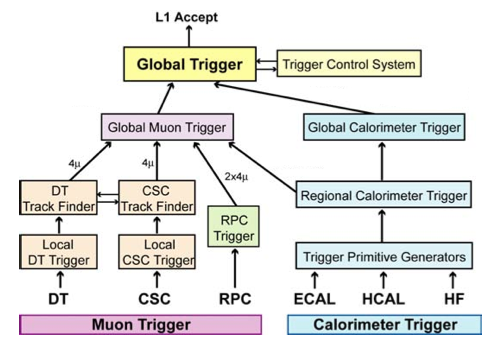
\includegraphics[width=\textwidth]{figs/trigger2}
  \caption{An overview of the CMS L1 trigger where the detector inputs are at the bottom and the subsequent steps in rate reduction proceed vertically upwards.~\cite{Halyo:2013iba}}
  \label{fig:L1T}
\end{figure}

Following the receipt of an L1 accept, a readout of the front-end electronics signals is performed and events are then processed by the HLT, the second tier of the CMS trigger. The entire CMS HLT system is implemented in a single processor cluster farm comprised of commercial computers running Linux. This so-called ``Event Filter Farm'' consists of three main components including the Readout Unit (RU), which is connected to the detector front-end readout and executes the primary step of data concentration by assembling fragments of an event from given detector partitions. Following this, the Builder Unit (BU) performs a full event assembly using the event fragments from the RUs, which are subsequently buffered while they proceed through the final event selection in the Filter Unit (FU)~\cite{Andre}. In order to satisfy the requirements of a high and inclusive selection efficiency for various physics objects, as well as maintain a rate of accepted events within $\mathcal{O}$(100) Hz, the HLT algorithms employed in the FU are as close as possible to those used in standard offline reconstruction. 

In order to strike a balance between the fast rejection of uninteresting events and minimization of overall CPU usage, reconstruction and selection at the HLT level makes use of two steps which nearly resemble distinct trigger systems. Denoted as ``Level-2'' and ``Level-3'', the major distinction between the each step is the reconstruction of full tracks in the tracker used at Level-3, where Level-2 solely makes use of information from the calorimeter and muon systems. Track reconstruction requires significantly larger amounts of CPU time than the correlation of calorimeter and muon detector data owing to the high number of readout channels from the inner tracker, the complex pattern recognition algorithms, and the higher rate of combinatorics. 

In electron and photon selection, the Level-2 algorithms involve the clustering of energy deposits in the ECAL and the measurement of the cluster energy and position solely from the calorimetric information. Since electrons radiate in the material between the interaction point and the ECAL, and the 4T magnetic field causes bending, the spray of radiated energy reaches the ECAL. The Level-2 algorithm reconstructs the electron energy by clustering cells along a $\phi$ road, since the radiated spray of energy from the electron is contained in the $\phi$ direction, to a good approximation. The following step is termed as ``Level-2.5'' since only partial as opposed to full tracking information is employed, such that superclusters (groups of energy clusters along the $\phi$ direction) are matched to hits within the pixel detector. Precise electron position and momentum can be determined solely by using the pixel hits, since most of the tracker material proceeds the pixel layers hence any photon conversions usually take place after these layers. This matching step further divides the electromagnetic triggers into two streams: one for electron candidates and one for photon candidates, which pass much higher energy threshold requirements. At the final stage, the ``Level-3'' step involves a full track reconstruction which is seeded by the hits in the pixel layers from the previous step. At this stage, consistency of the energy and momentum measurements (E/p) and consistency of the track position with the ECAL hit position is required. In the endcaps, requirements on the fraction of energy found behind the ECAL supercluster (in the HCAL) over the supercluster energy (H/E) is made in order to discriminate hadronic activity (i.e. $\pi^{0}$) from $e/\gamma$ candidates. 

For muon selection requirements at the HLT level, the Level-2 algorithm is seeded by the maximum of four muon candidates found by the L1 GMT and employs the digitized hits in the muon detectors to reconstruct and verify the trajectories that lead to the L1 accept. Tracks are reconstructed according to the Kalman filter technique, described in greater detail in~\cite{Fruhwirth:1987fm}, which ameliorates the \pt measurement from L1. Isolation criteria on the basis of the calorimetric energy sum contained within a cone around the muon candidate can be applied at Level-2. The defining feature of the Level-3 muon selection, is the addition of silicon tracker hits to the trajectory which further refines the \pt measurement and provides a sharper trigger threshold. At this final stage, the number of pixel tracks in a region around the muon trajectory projected towards the inner detector can be used to suppress contributions from non-prompt muon decays of b, c, $\pi$ and K particles.

The HLT algorithm for jet selection is a simplified version of the more involved offline algorithms described in the following chapter dedicated to object reconstruction. The algorithm requires the organization of calorimeter data into towers for which the HCAL segmentation in $\eta \times \phi$ is $0.0875\times 0.0875$ in the barrel and approaches an $\eta$ segmentation of 0.0175 near the edges of the endcaps. Correspondingly, for each HCAL barrel tower, there are approximately 25 ECAL crystals, whereas in the endcap regions the crystal number varies with $\eta$. The basic iterative algorithm for jet finding at HLT consists of designating a ``seed tower'' which has the highest tower \Et, and using this to calculate the direction of the ``protojet''. By determining the transverse-energy-weighted angles of the towers in a cone around the protojet in $\eta-\phi$ space, the direction measurement of the seed protojet is updated and the energy in the cone is summed to obtain the protojet \Et. The procedure is repeated until the protojet energy changes by less than $1\%$ between iterations and the direction in $\Delta\eta^2+\Delta\phi^2$ space changes by less than 0.01, or on the other hand, 100 iterations have been completed. Towers that are associated with a stable protojet found after this procedure are removed from the listed sorted by descending tower \Et, and the entire jet finding procedure is repeated until no objects remain in the list or conversely, the tower with the highest \Et is below a preset ``seed'' threshold dictated by the algorithm. More details on the respective parameters such as cone-size, seed energy threshold, and minimum jet energy threshold can be found in~\cite{Cittolin:578006}.

The ability to use simple trigger requirements to attain high efficiencies for most physics objects is a key feature of the HLT system, along with the flexibility it allows for the modification of existing trigger thresholds or the addition of new triggers should the available computing bandwidth allow for such options. Using a single processor farm, the HLT selection of 1:1000 is achieved and subsequently the data are transmitted to the online and offline computing services.

\subsection{Computing and data storage}
\label{subsec:computing}

\begin{figure}
  \centering
  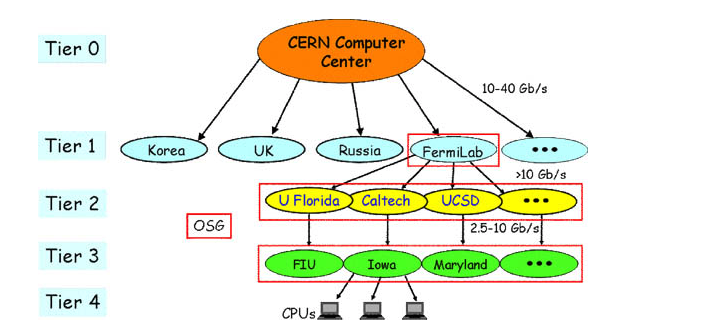
\includegraphics[width=\textwidth]{figs/computing}
  \caption{A flow chart of the multi-tier worldwide LHC computing grid, where the components circled in red are examples of the U.S. resources that are part of Open Science Grid (OSG) as defined in detail in~\cite{FM1866}. The computing resources at Northwestern University fall under the Tier 3 computing category.}
\label{fig:computing}
\end{figure}

The events selected by the HLT for physics analysis, along with events that are selected for calibration purposes, and a fraction of events rejected by the HLT are then processed either online or transmitted to the offline systems for event reconstruction, selection, and any other offline processing. The HLT farm writes ``raw'' data events of $\mathcal{O}$(1.5) MB size at an approximate rate of 100 Hz which are grouped into primary datasets based on HLT trigger object requirements and organized into $\mathcal{O}(10)$ online streams to be processed offline. The raw data is processed at CERN's Tier-0 farm where events are reconstructed with timescales ranging from a few to 24 hours depending on the level of priority. The Tier-0 farm writes out ``reco'' data events of $\mathcal{O}$(0.25) MB size to one of approximately 6 Tier-1 sites, which produce Analysis Object Data (AOD) events of $\mathcal{O}$(0.5) MB~\cite{Eck:840543}. The AOD events are derived from reco events and contain a copy of the high-level physics objects along with a summary of reco information which enable additional analysis handles such as track refitting. In 2014, in an effort to reduce the event size while simultaneously retaining all the necessary data from the AOD data formats, a MiniAOD format~\cite{1742-6596-664-7-072052} was introduced as a derivation from the AOD. MiniAOD event sizes are of $\mathcal{O}$(0.05) MB and contian high-level physics objects, along with Particle Flow candidates which are described in the following chapter, and information from the simulated particles. At this stage, the MiniAOD data format can be skimmed according to the objects and selection necessary for data analysis. The multi-tier worldwide LHC computing grid shown in~\FigureRef{fig:computing} displays the full computing chain down to the individual CPUs employed by the end-user, the analyzer.
